\documentclass[11pt]{report}
\usepackage[letterpaper, total={6.5in, 10in}]{geometry}
%\usepackage{fancyhdr}
%\pagestyle{fancy}
\usepackage{amsmath, amsthm, mathpazo, epic, eepic, color, array}
\usepackage{amssymb}
%\usepackage{graphicx}
\usepackage{cancel}
\usepackage{pgfplots}
\usepackage{multicol}
\pgfplotsset{compat=1.13}
\usepackage{etoolbox}
\makeatletter
\patchcmd{\chapter}{\if@openright\cleardoublepage\else\clearpage\fi}{}{}{}
\makeatother
\usepackage{hyperref}

\usepackage{enumerate}
\usepackage{enumitem}

\usepackage{tikz}
\usetikzlibrary{positioning,chains,fit,shapes,calc,arrows,patterns}
\usepackage{tkz-graph}
\usetikzlibrary{arrows, petri, topaths}
\usepackage{tkz-berge}
\usepackage[all]{xy}
\usepackage{textcomp}

\newboolean{colorprint}
\setboolean{colorprint}{true}
%\setboolean{colorprint}{false}

\ifthenelse{\boolean{colorprint}}{%
\newcommand{\colorone}{blue}
\newcommand{\colortwo}{red}
\newcommand{\coloronefill}{blue!15!white}
\newcommand{\colortwofill}{red!15!white}
\newcommand{\colormapone}{rgb=(.4,.4,1); rgb=(.8,.8,1)}
\newcommand{\colormaptwo}{rgb=(1,.4,.4); rgb=(1,.8,.8)}
\newcommand{\colormapplaneone}{rgb=(.7,.7,1); rgb=(.9,.9,1)}
\definecolor{colormaponebottom}{rgb}{.4,.4,1}
\definecolor{colormaponetop}{rgb}{.8,.8,1}
\definecolor{colormaptwobottom}{rgb}{1,.4,.4}
\definecolor{colormaptwotop}{rgb}{1,.8,.8}
}% ends color
{% not color
\newcommand{\colorone}{black}
\newcommand{\colortwo}{black!50!white}
\newcommand{\coloronefill}{black!15!white}
\newcommand{\colortwofill}{black!05!white}
\newcommand{\colormapone}{rgb=(.4,.4,.4); rgb=(.7,.7,.7)}
\newcommand{\colormaptwo}{rgb=(.6,.6,.6); rgb=(.9,.9,.9)}
\newcommand{\colormapplaneone}{rgb=(.8,.8,.8); rgb=(.95,.95,.95)}
\definecolor{colormaponebottom}{rgb}{.4,.4,.4}
\definecolor{colormaponetop}{rgb}{.7,.7,.7}
\definecolor{colormaptwobottom}{rgb}{.6,.6,.6}
\definecolor{colormaptwotop}{rgb}{.9,.9,.9}
}%

\newlength\tindent
\setlength{\tindent}{\parindent}
\setlength{\parindent}{0pt}
\renewcommand{\indent}{\hspace*{\tindent}}

\pgfplotsset{my style/.append style={axis x line=middle, axis y line=
middle, xlabel={$x$}, ylabel={$y$}, axis equal }}

\pgfplotsset{compat=1.13}

\begin{document}

{\bf Chapter 2: Derivatives}\\

%%%%%%%%%%%%%%%%%%%%%%Section 2.1%%%%%%%%%%%%%%%
{\bf Section 2.1 Instantaneous Rates of Change: The Derivative}
\vskip .25 truein

All page numbers refer to original APEX text page numbers.\\
\\

\textbf{p. 57,} Paragraph 2 typo: "...150 feet. Students of physics..."

\vskip 1 truecm

\textbf{p. 58} \\

Move current Figure 2.1 up then add this graph in the margin near difference quotient - refer to it as Figure 2.2 in text (then current Figure 2.2 becomes 2.3, etc)\\
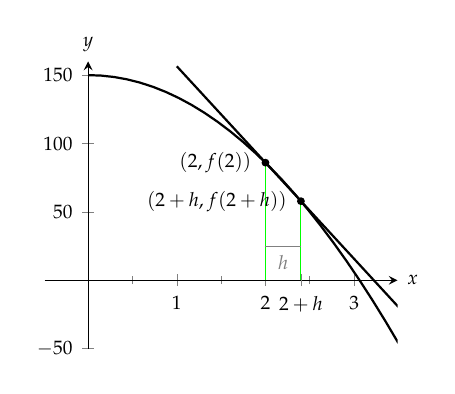
\begin{tikzpicture}
%I removed this comman from APEX code you sent me so I could see the graph when I texed it: width=\marginparwidth
\begin{axis}[width=.5\textwidth,tick label style={font=\scriptsize},
minor x tick num=1,
axis y line=middle,axis x line=middle,ymin=-50,ymax=160,xmin=-.49,xmax=3.49,
name=myplot, extra x ticks={2.4}, extra x tick labels={$2+h$}]
\addplot [{\colorone},domain=0:3.5,thick] {150-16*x*x};
\addplot [{\colortwo},domain=1:3.5,thick] {(90.75-28.16*x)/.4};
\draw[green] (2,0)--(2,86);
\draw[green] (2.4,0)--(2.4,57.84); 
\draw[gray] (2,25)--(2.4,25) node[pos=0.5, below]{\scriptsize $h$};
\node[label={180:{\scriptsize $(2,f(2))$}},circle,fill,inner sep=1pt] at (axis cs:2,86) {};
\node[label={180:{\scriptsize $(2+h,f(2+h))$}},circle,fill,inner sep=1pt] at (axis cs:2.4,57.84) {};
\end{axis}
\node [right] at (myplot.right of origin) {\scriptsize $x$};
\node [above] at (myplot.above origin) {\scriptsize $y$};
\end{tikzpicture}\\
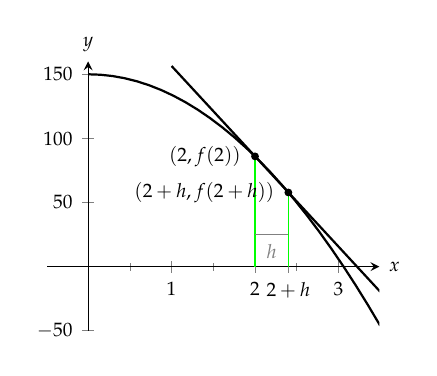
\begin{tikzpicture}
\begin{axis}[width=165pt,tick label style={font=\scriptsize},minor x tick num=1,
axis y line=middle,axis x line=middle,ymin=-50,ymax=160,xmin=-.49,xmax=3.49,
name=myplot, extra x ticks={2.4}, extra x tick labels={$2+h$}]
\addplot [{\colorone},domain=0:3.5,thick] {150-16*x*x};
\addplot [{\colortwo},domain=1:3.5,thick] {(90.75-28.16*x)/.4};
\draw[green] (2,0)--(2,86);
\draw[green] (2.4,0)--(2.4,57.84); 
\draw[gray] (2,25)--(2.4,25) node[pos=0.5, below]{\scriptsize $h$};
\node[label={180:{\scriptsize $(2,f(2))$}},circle,fill,inner sep=1pt] at (axis cs:2,86) {};
\node[label={180:{\scriptsize $(2+h,f(2+h))$}},circle,fill,inner sep=1pt] at (axis cs:2.4,57.84) {};
\end{axis}
\node [right] at (myplot.right of origin) {\scriptsize $x$};
\node [above] at (myplot.above origin) {\scriptsize $y$};
\end{tikzpicture}\\

Below the difference quotient replace "where h is small" with "where $h$ is the change in time after $2$ seconds."
\vskip 1 truecm

\textbf{p. 59} \\ 
If space under Figure 2.2 (soon to be 2.3) is still there try to remove it.\vskip 1 truecm

\textbf{p. 60} \\ 
In "Definition 7 Derivative at a Point" box:
Move the text "If the limit exists, we say that $f$ is differentiable... then f is differentiable on $I$." outside of the box - between Def 7 \& Tangent Line definition.
 \vskip 1 truecm

\textbf{pp. 61 - 62} \\ 
Cut "Another important line that can be created...Definition 9 Normal Line...Example 33" and all text related to this topic \& remove Figure 2.4. 
\vskip 1 truecm

\textbf{p. 65} \\ 
Example 37: in the sentence, "Now find common denominator..." replace "pull" with "factor.
\vskip 1 truecm

\textbf{p. 66} \\ 
Example 38 delete ! after $=\cos x$. \vskip 1 truecm
\textbf{Tim - I don't like the length of the positive x-axis but it needed to be that long to see the label for cos x. Do you know of another way to do this?}\\
%%http://tex.stackexchange.com/questions/34939/axis-with-trigonometric-labels-in-pgfplots%%%

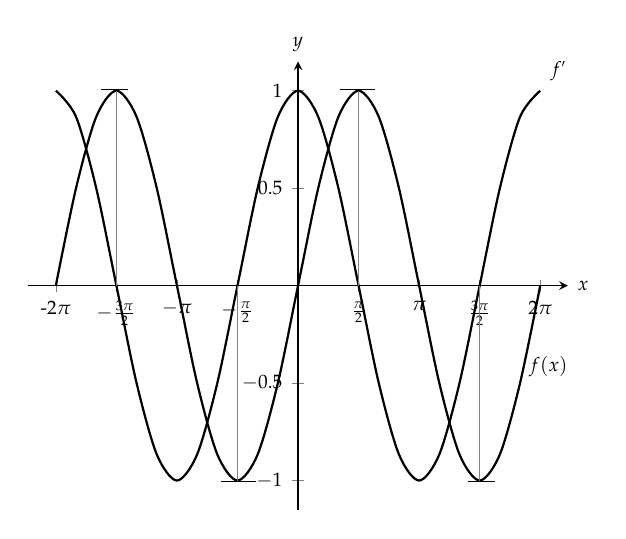
\begin{tikzpicture}
%I removed this comman from APEX code you sent me so I could see the graph when I texed it: width=\marginparwidth,
\begin{axis}[tick label style={font=\scriptsize}, axis y line=middle,axis x line=middle, ymin=-1.15, ymax=1.15,xmin=-7,xmax=7,name=myplot,  xtick={-6.28318, -4.7123889, -3.14159, -1.5708, 1.5708, 3.14159, 4.7123889, 6.28318}, xticklabels={-$2\pi$, $-\frac{3\pi}{2}$,$-\pi$, $-\frac{\pi}{2}$, $\frac{\pi}{2}$,$\pi$, $\frac{3\pi}{2}$, $2\pi$}]
\addplot [{\colorone}, smooth, domain=-6.28318:6.28318,thick] {sin(deg(x))} 
         node [pos=.95, above right] {\scriptsize $f(x)=\sin{x}$};
\addplot [{\colortwo},smooth, domain=-6.28318:6.28318,thick] {cos(deg(x))}
         node [pos=1, above right] {\scriptsize $f'(x)=\cos{x}$};
\draw[\colortwo] (-5.1,1.005)--(-4.4,1.005);
\draw[\colortwo] (-2,-1.005)--(-1.1,-1.005);
\draw[\colortwo] (5.1,-1.005)--(4.4,-1.005);
\draw[\colortwo] (2,1.005)--(1.1,1.005);  
\draw[gray] (-4.7123889,0)--(-4.7123889,1);
\draw[gray] (-1.5708,0)--(-1.5708,-1);
\draw[gray] (1.5708,0)--(1.5708,1);
\draw[gray] (4.7123889,0)--(4.7123889,-1);
\end{axis}
\node [right] at (myplot.right of origin) {\scriptsize $x$};
\node [above] at (myplot.above origin) {\scriptsize $y$};
\end{tikzpicture}\\
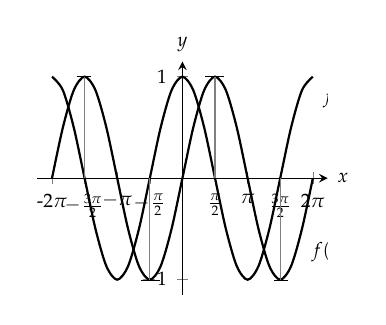
\begin{tikzpicture}
\begin{axis}[width=150pt,tick label style={font=\scriptsize}, axis y line=middle,axis x line=middle, ymin=-1.15, ymax=1.15,xmin=-7,xmax=7,name=myplot,  xtick={-6.28318, -4.7123889, -3.14159, -1.5708, 1.5708, 3.14159, 4.7123889, 6.28318}, xticklabels={-$2\pi$, $-\frac{3\pi}{2}$,$-\pi$, $-\frac{\pi}{2}$, $\frac{\pi}{2}$,$\pi$, $\frac{3\pi}{2}$, $2\pi$}]
\addplot [{\colorone}, smooth, domain=-6.28318:6.28318,thick] {sin(deg(x))} 
         node [pos=.95, below right] {\scriptsize $f(x)=\sin{x}$};
\addplot [{\colortwo},smooth, domain=-6.28318:6.28318,thick] {cos(deg(x))}
         node [pos=1, below right] {\scriptsize $f'(x)=\cos{x}$};
\draw[\colortwo] (-5.1,1.005)--(-4.4,1.005);
\draw[\colortwo] (-2,-1.005)--(-1.1,-1.005);
\draw[\colortwo] (5.1,-1.005)--(4.4,-1.005);
\draw[\colortwo] (2,1.005)--(1.1,1.005);  
\draw[gray] (-4.7123889,0)--(-4.7123889,1);
\draw[gray] (-1.5708,0)--(-1.5708,-1);
\draw[gray] (1.5708,0)--(1.5708,1);
\draw[gray] (4.7123889,0)--(4.7123889,-1);
\end{axis}
\node [right] at (myplot.right of origin) {\scriptsize $x$};
\node [above] at (myplot.above origin) {\scriptsize $y$};
\end{tikzpicture}
\hspace{1in}
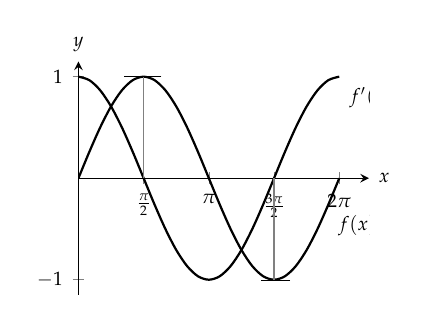
\begin{tikzpicture}
\begin{axis}[width=150pt,tick label style={font=\scriptsize}, axis y line=middle,axis x line=middle, ymin=-1.15, ymax=1.15,xmin=0,xmax=7,name=myplot,  xtick={1.5708, 3.14159, 4.7123889, 6.28318}, xticklabels={$\frac{\pi}{2}$,$\pi$, $\frac{3\pi}{2}$, $2\pi$}]
\addplot [{\colorone}, smooth, domain=0:6.28318,thick] {sin(deg(x))} 
         node [pos=.95, below right] {\scriptsize $f(x)=\sin{x}$};
\addplot [{\colortwo},smooth, domain=0:6.28318,thick] {cos(deg(x))}
         node [pos=1, below right] {\scriptsize $f'(x)=\cos{x}$};
%\draw[\colortwo] (-5.1,1.005)--(-4.4,1.005);
%\draw[\colortwo] (-2,-1.005)--(-1.1,-1.005);
\draw[\colortwo] (5.1,-1.005)--(4.4,-1.005);
\draw[\colortwo] (2,1.005)--(1.1,1.005);  
%\draw[gray] (-4.7123889,0)--(-4.7123889,1);
%\draw[gray] (-1.5708,0)--(-1.5708,-1);
\draw[gray] (1.5708,0)--(1.5708,1);
\draw[gray] (4.7123889,0)--(4.7123889,-1);
\end{axis}
\node [right] at (myplot.right of origin) {\scriptsize $x$};
\node [above] at (myplot.above origin) {\scriptsize $y$};
\end{tikzpicture}\\
The figure label could be: Figure WHATEVER: The function $f(x)=\sin x$ and its derivative $f'(x)=\cos x$.\\

\vskip .5 truecm
This picture should go next to this paragraph that replaces the paragraph beginning with "We have found that when...": \vskip .25 truecm
We have found that when $f(x) = \sin x, f'(x) = \cos x$ (see Figure WHATEVER). Initially, this might be somewhat surprising; the result of a tedious limit process and the sine function is a nice function. Then again, perhaps this is not entirely surprising. The sine function is periodic - it repeats itself on regular intervals. Therefore its rate of change also repeats itself on the same regular intervals. In fact, if we think about $f'(x)$ as the slope of the tangent to the sine curve we notice the following\\
\begin{itemize}
\item if the slope of tangent lines is 0 then $f'(x)=\cos x$ crosses the $x-$axis;
\item if the slopes of the tangent lines are positive then $f'$ lies above the $x-$axis; and 
\item if the slopes of the tangent lines are negative then $f'$ lies below the $x-$axis.
\end{itemize}

We should have known the derivative would be periodic; we now know exactly which periodic function it is.\\
\vskip 1 truecm

\textbf{p. 67} \\ 
Insert bracketed word [ ]: in paragrah starting with "Since $x=0$ is the point where our function's definition switches from one piece to [the] other,..."
\vskip 1 truecm

\textbf{p. 68} \\ 
In Solution at topic of page change $\displaystyle{\lim_{x\to 0}}$ of the difference quotients to $\displaystyle{\lim_{h\to 0}}$.
\vskip 1 truecm

\textbf{Exercises 2.1}\\
For exercises $6 - 12$ change the directions to:\\
In exercises $6 - ??$ (a) use the definition of the derivative to compute the derivative function.
(b) Find the tangent line to the graph of the given function at $x=c$.
 
The problems should appear in the following order. \#6-9 are the same as before. I added problems 10, 12, and 14 and all independent variables are $x$:\\
6.  $f(x)=6$ at $x=-2$\vskip .25 truecm
7.  $f(x)=2x$ at $x=3$\vskip .25 truecm
8.  $f(t)=4-3x$ at $x=7$\vskip .25 truecm
9.  $g(x)=x^2$ at $x=-2$\vskip .25 truecm
10. $h(x)=2x-x^2$ at $x=1$\vskip .25 truecm
11. $f(x)=3x^2-x+4$ at $x=-1$\vskip .25 truecm
12. $g(x)=\sqrt {x+3}$ at $x=1$\vskip .25 truecm
13. $\displaystyle{r(x)={1 \over x}}$ at $x=-2$\vskip .25 truecm
14. $\displaystyle{h(x)=\frac{3}{\sqrt {x}}}$ at $x=4$\vskip .25 truecm
15. $\displaystyle{f(x)=\frac {1}{x-2}}$ at $x=3$\vskip .25 truecm

\textbf{Answers} \vskip .25 truecm
7.   (a) Same as current \\
      (b)   $y=2x$      \vskip .25 truecm
9.   (a) Same as current \\
      (b)   $y=-4x-4$   \vskip .25 truecm
11.  (a)   $f'(x)=6x-1$\\
      (b)    $y=-7x+1$\vskip .25 truecm
13.  (a) Same as current \\
      (b)   $y=-\frac{1}{4}x-1$ \vskip .25 truecm
15.  (a) Same as current \\ 
      (b)    $y=-x+4$    \vskip .5 truecm

New section of problems:\\
Each limit represents the derivative of some function, $f$, at some number $c$. State an appropriate $f$ and $c$ for each.\vskip .25 truecm
16.  $\displaystyle{\lim_{h\to 0}} \frac{\sqrt {16+h} - 4}{h}$   \vskip .25 truecm
17.  $\displaystyle{\lim_{h\to 0}} \frac{(3+h)^4-81}{h}$   \vskip .25 truecm
18.  $\displaystyle{\lim_{h\to 0}} \frac{\frac{1}{x+h}-2}{h}$   \vskip .25 truecm
19.  $\displaystyle{\lim_{h\to 0}} \frac{\cos (-\pi +h)+1}{h}$   \vskip .25 truecm

\textbf{Answers} \vskip .25 truecm
17.  $f(x) = \sqrt x, c = 16$ \vskip .25 truecm
19.  $\frac{1}{x}, c = \frac{1}{2}$ \vskip .5 truecm


After current \#20 (still \#20) insert new \#21 $f(x) = \sqrt x, x=4$

\end {document}
